% just setup stuff
\documentclass[12pt]{article}

% Alter some LaTeX defaults for better treatment of figures:
    % See p.105 of "TeX Unbound" for suggested values.
    % See pp. 199-200 of Lamport's "LaTeX" book for details.
    %   General parameters, for ALL pages:
    \renewcommand{\topfraction}{0.9}	% max fraction of floats at top
    \renewcommand{\bottomfraction}{0.8}	% max fraction of floats at bottom
    %   Parameters for TEXT pages (not float pages):
    \setcounter{topnumber}{2}
    \setcounter{bottomnumber}{2}
    \setcounter{totalnumber}{4}     % 2 may work better
    \setcounter{dbltopnumber}{2}    % for 2-column pages
    \renewcommand{\dbltopfraction}{0.9}	% fit big float above 2-col. text
    \renewcommand{\textfraction}{0.07}	% allow minimal text w. figs
    %   Parameters for FLOAT pages (not text pages):
    \renewcommand{\floatpagefraction}{0.7}	% require fuller float pages
	% N.B.: floatpagefraction MUST be less than topfraction !!
    \renewcommand{\dblfloatpagefraction}{0.7}	% require fuller float pages

	% remember to use [htp] or [htpb] for placement

% style, margins, etc...
\usepackage[left=0.5in,top=1.5in,right=0.5in,bottom=1.5in]{geometry}
\usepackage{graphicx}
\usepackage{amsmath}
\usepackage{listings}
	\lstset{language = C}
\usepackage{url}
% all figures are stored in the subdir "figs"
\graphicspath{{./figs/}}

% define the title and author(s)
\author{Peter Bilodeau\\
	peterjbilodeau@gmail.com\and
	Brady Butler\\
	m.brady.butler@gmail.com\and
	Breanna Stanaway\and
	Cody Morgan\\
	}
\title{ECE 477 Final Project}

\begin{document}

%--------------------------------------------------------------------------
% generates the title
\maketitle

% abstract
\begin{abstract}

This report discusses the design of a quadrocoptor. 

\end{abstract}
\clearpage

% start a new page
\clearpage

% generates the table of contents
%(need to run latex twice for this to get updated)
\tableofcontents

% start a new page
\clearpage

%--------------------------------------------------------------------------
% The Actual Paper

\section{Introduction}

For this project, we designed and built an autonomous flying quadrotor.  Our design anticipates automatic stability control and navigation. This project lays the foundation for integrated sensor and motor control systems.
We built a custom aluminum frame and a custom electronic main board, and use stock hobby motors, propellers and lithium-polymer battery.


\clearpage
\section{Flight Dynamics}
	To begin, it is important to understand the basic of quadrotor flight dynamics.  A quadrotor has six degrees of freedom.  Two in the horizontal plane (forward/back and left/right), one vertically (altitude), and 3 axes of rotation.  We decided to define on of the four rotors as the 'front' of the craft.  This rotor we call 'north'; the others are 'south,' 'east,' and 'west' respectively.  Some designs define a pair of rotors as the front.  This is known as flying 'X' mode as opposed to '+' mode like our project.  Using standard flight terminology, we defined three axes of rotation as follows: rotation about the vertical axis is called yaw, where counter-clockwise (turning left) is the positive direction, rotation about the horizontal axis perpendicular to the forward direction is called pitch, north rotor up (leaning back) is the positive direction, finally, rotation about the horizontal axis parallel to the forward direction is called roll, where leaning left is the positive direction.
	Adjusting the roll and pitch of the craft in flight is fairly straightforward.  If one rotor is lower than the others, then the quadrotor is leaning in that direction.  We can increase the thrust of that motor to compensate and level out.  Yaw, on the other hand, is slightly more complicated.  We use 2 pair of propellers rotating in opposite directions.  Each pair, then, generates a torque opposing that of the other pair.  We can then rotate in the yaw direction by speeding up one set of rotors with respect to the other.  Since simply speeding up two of the motors will generate more overall lift, the quadrotor will fly up.  Thus we need to reduce the thrust of the opposite pair of rotors at the same time as we increase the thrust of the other pair.  This will keep the over thrust constant, while still causing a yaw rotation.  Similarly, when correcting roll and pitch, we decrease the thrust of the higher rotor at the same time we increase the thrust of the lower one.  What the controls really adjust then, is the relative speed of opposing rotors or pairs of rotors.


\clearpage
\section{System Architecture}

The quadrotor control board integrates several distinct systems.  


\clearpage
\section{Motor Control}



\clearpage
\section{Power}



\clearpage
\section{Communication}



\clearpage
%This document for talking about the different sensors.
\section{Sensors}
To create a stable system different aspects of the flight were monitored using sensors. Section \ref{Together} discusses the integration of all sensors to create an attitude. Section \ref{Nun} discusses the Nunchuck. Section \ref{Sonar} discusses the sonar. 

\section{Sensors}

\subsection{Wii Nunchuck 3-Axis Accelerometer}

\paragraph{}
The Wii Nunchuck accelerometer is an I^{2}C device that provides 10 bits of data representing the magnitude of acceleration in each of the x, y, and z axes.  The data obtained from the accelerometer form the foundation of the roll and pitch estimations for the quadrotor.  The I^{2}C write address of the accelerometer is 0xA4 while the read address is 0xA5.  All code related to the accelerometer can be found in the {\it nunchuck.h} header file.

\paragraph{Initialization}
Before it can be used, the device must first be initialized in one of two different ways.  The first method involves simply writing the value 0x00 to address 0xA4 of the accelerometer.  This will cause the device to send back encrypted data that must be decrypted before it can be used.  Since we sought to poll the sensory devices, calculate the new motor values, and then update the quadrotor as fast as possible, we chose to forgo the encryption route.

\paragraph{}
The second initialization is accomplished by writing the value 0x55 to device address 0xF0 and then writing the value 0x00 to address 0xFB.  This will put the device in unencrypted mode and allow all data to be immediately useable as it comes back from the accelerometer.  We initialize our quadrotor this way using the {\bf power_on_nunchuck()} function.

\paragraph{Reading the Data}
Once a read is initiated, data comes back from the accelerometer in six byte chunks.  The first two bytes pertain to the position of the previously attached joystick and are ignored for the purposes of this project.  The next three bytes that come from the device are the x, y, and z axis 8 MSB, respectively.  The final byte contains the 2 LSB for each axis as well as button press data for the two buttons that were previously attached as part of the Wii nunchuck.  For each axis, to reconstitute the data, we left shift the 8 MSB two places and then OR that result with the 2 LSB to yields the full 10 bit resolution.  The accelerometer data read and reconstitution is accomplished via the {\bf get_data_nunchuck()} function..  It is important to note that within this function, {\bf send_zero_nunchuck()} is called, which simply sends the value 0x00 to the device.  This must be done after each data read or the accelerometer will stop responding to read requests.

\paragraph{Interpreting the Data}
The 10 bit value of each axis retrieved from the accelerometer is an unsigned integer representing the magnitude of that distinct axis.  Since the 10 bit value is unsigned with a range between 0 and 1023, each axis has a characteristic offset so that the zero value falls close to the middle of the range.  These values were determined for the x and y axes by reading the raw values from the accelerometer while the device was flat and stationary (thus experiencing zero x and y acceleration).  Once acquired, we hardcoded these values using defines in the header file.  The z axis was not calibrated since it was not needed for attitude calculation, as will be explained in the subsequent paragraph.

\paragraph{}
Calculating the attitude of the quadrotor using the accelerometer presented a challenge because it involved a significant amount of trig operations, which are expensive in general; especially on the AVR.  Therefore we decided to use the small angle approximation which gives a value within 5% of the actual angle up to 30$^\circ$.  To do this, we measured the maximum value given by the accelerometer for the x and y axes (i.e. when acceleration for each axis was at a maximum) and then used the following equation to obtain the quadrotor's roll and pitch, respectively.
\begin{equation}
\theta = \frac{axis_value}{axis_max}\times\frac{180}{\pi}
\end{equation}
This method was sufficient to accurately predict the roll and pitch of the quadrotor for angles up to 35$^\circ$.
 
\subsection{2-axis Gyroscope}

\paragraph{}
The 2-axis gyroscope requires Analog-to-Digital Conversion (ADC) and gives a rotational velocity in degrees per second about the x and y axes.  This data was used to help smooth out the roll and pitch measurements derived from the data given by the 3-axis accelerometer.  All code related to the gyroscope can be found in the {\it gyro.h} header file.

\paragraph{Setting up the ADC}
A previous lab addressed the specifics of performing ADC on the AVR.  The ADC used for the quadrotor is not significantly different.  Since the 2-axis gyro has two different analog outputs, the  x and y outputs are connected to ADC Channels 0 and 1 on the AVR, respectively.  The only major difference between the use of ADC in that lab and the use of ADC for the quadrotor is that we chose to use the AREF pin to provide a reference voltage of 3.3V.  We only learned of the danger in using this method after our quadrotor was already built, otherwise we would have used the AV_{CC} as a reference voltage.  AREF mode is set by clearing the REFS1:0 bits of the ADMUX register.

\paragraph{Triggering and Reading the Conversion}
 An ADC is triggered by writing a 1 to the ADSC bit of the ADCSRA register.  We handle the reading of the data through the {\it ADC_vect} interrupt.  When the interrupt is triggered, we read the 8 LSB from the ADCL register followed by the 2 MSB from the ADCH register.  Just like the accelerometer, the gyroscope also has a bias that must be taken into account.  We measured the bias of each axis when the gyroscope was at rest and then hardcoded the values in using defines.  When we do calculations, the bias is subtracted to give the true rotational velocity.

\paragraph{}
One other important thing to note is that gyroscope actually has four different outputs.  It has the standard x and y axis (roll and pitch, respectively), but it also has two other channels for High Resolution Mode.  These high resolution outputs are 4.5 times more sensitive to change than the standard outputs.  We do not use these outputs from the gyroscope, but our code is capable of handling them through the use of a ternary operation in the interrupt vector where the gyroscope value is multiplied by a scaling factor to give degrees per second.  Once the value is converted to this form, we check which channel was being used, x or y axis, and then put the data into the proper sensor data cache variable.  Finally, we switch the ADC channel to the other axis by toggling the LSB of the ADMUX register so that we alternate between reading the x and y axis rotational velocity from the gyroscope.

\subsection{3-axis Magnetometer}

\paragraph{}
The magnetometer is an I^{2}C device that provides three 16 bit values representing the magnitude of the magnetic field along the x, y and z axes.  This information is used to measure the heading of the quadrotor.  In future iterations, this heading data will be used to correct for yaw.  The I^{2}C write address of the magnetometer is 0x3C while the read address is 0x3C.  All code related to the magnetometer can be found in the {\it magnetometer.h} header file.

\paragraph{Initialization}
Before the magnetometer can be used, it must be initialized by writing three bytes to the device.  First, the value 0x70 must be written to device address 0x00.  Then the value 0x01 must written to device address 0xA0.  Finally, the value 0x02 must be written to device address 0x00.  Once this is done, the magnetometer is ready to be used.  This process is handled on the quadrotor by the {/bf power_on_magnetometer()} function.

\paragraph{Reading and Interpreting the Data}
Data is read from the magnetometer by writing the address 0x03 to the device, and then performing a 6 byte read.  The bytes that come back are the 8 MSB, followed by the 8 LSB of the x, y, and z axes, respectively.  This data does not have any offset that needs to be taken into account.  Instead, the three values are the x, y, and z components of a vector pointing towards Magnetic North.  The {\bf compensate_for_tilt()} function uses these three raw vector values, as well as the current roll and pitch values, to give the heading of the  quadrotor in degrees.  The {\bf get_data_magnetometer()} function performs the 6 byte read, calls the conversion function, and then puts the heading value into the {\bf compass_heading} component of the {\bf sensor_data_cache}.

\subsection{Barometer}

\paragraph{}
We had originally planned on using a barometer for altitude readings.  But the device arrived with calibration values that were outside of the acceptable range as set by the manufacturer, thus indicating a defective item.  We wrote all of the code before actually checking the EEPROM burned calibration values, so there is a {\it barometer.h} header file that contains all of the code to use this device despite the fact that our quadrotor does not incorporate any of it.  The barometer is a standard I^{2}C device with a few peculiarities.  The device must have a control byte written to it to start a pressure or temperature reading, and then it requires 4.5 {\it ms} before the value can actually be read.  That is a very long time to wait in term of updating the motor values, so maybe is was best that this device was broken.

\subsection{Sonar}

\paragraph{}
To handle the altitude reading of our quadrotor we used a sonar device.  The sonar device is not, like most of our devices, I^{2}C.  Instead, it gives a rising edge on its output pin when it sends out a sound wave, and then gives a falling edge on its output pin when the wave returns.  Thus in order for the sonar device to be used, we needed two compare values and an input capture interrupt on a single clock.  Since the clocks on our AVR were already being used for other things, we decided to put the sonar device on another AVR and then use that AVR as an I^{2}C slave.  All code related to the sonar can be found in the {\it sonar_slave.h} header file.

\paragraph{Initialization}
The sonar device, itself, does not need any initialization.  Instead, the AVR slave must be setup with the proper clock prescalar and interrupt mask to use input capture with the sonar device.  This is done within the {\bf setup_sonar()} function.  A prescalar of 8 is used with the 8 {\it MHz} to give a clock that counts in 1 $\mus$ increments.  The OCR1A value is set to 60000 so that the Timer 1 COMPA interrupt is called every 60 $\mus$.  The Timer mode is also set so that the clock resets when it hits the OCR1A value.  The OCR1B value is set to 5 so that the Timer 1 COMPB interrupt is called 5 $\mus$ after the COMPA interrupt.

\paragraph{Starting a Reading}
A sonar reading is triggered on the slave AVR every time the Timer 1 COMPA interrupt vector is called.  In this interrupt, PORTB is set to output mode and then Pin 0 is set high.  5 $\mus$ later the Timer 1 COMPB interrupt vector is called which sets Pin 0 low and changed PORTB to input mode.  This interrupt also sets the {\bf WAITINGFORECHO} flag which indicates that a sonar reading is in progress.  The 5 $\mus$ long pulse triggers the sonar device to send out a sound wave and thus Pin 0 needs to start listening for a rising edge from the sonar device.  The input capture interrupt catches the rising edge of the sonar device, notes the time, and then starts listening for a falling edge.  When the falling edge is captured, the $\Delta time$ is calculated and then the sonar distance in feet is calculated via the formula:
\begin{equation}
distance = frac{\Delta time \times 1130}{1000000}
\end{equation}



\subsection{Attitude \label{Together}}
\subsection{Nunchuck\label{Nun}}
\subsection{Sonar\label{Sonar}}
\subsection{GPS}
\subsection{}



\clearpage
\section{Data Filtering}

\paragraph{}
The data coming in from our sensory devices was capable of getting quite noisy.  Considering that the quadrotor is always moving and shaking when in flight, it was necessary to smooth out the data using a filtering scheme.  The altitude and attitude calculations were smoothed out using two separate methods.  Data filtering is handled through functions located in the {\it data.h} header file.

\subsection{Altitude}

\paragraph{}
Every time an altitude reading is obtained by querying the slave AVR, the master AVR calls {\bf update\_adj\_alt()}.  This function takes a weighted average of the old altitude reading and the new altitude reading before assigning this value as the new altitude.  The weighted average is expressed below:
\begin{equation}
new\_altitude = 0.75 \times old\_altitude + 0.25 \times new\_altitude\_reading
\end{equation}

\subsection{Attitude \label{attitude}}

\paragraph{}
The attitude calculations (i.e. roll and pitch) are smoothed out using a method called a Complementary Filter contained within the {\bf update\_adj\_rp()} function.  This function is called every time a new roll and pitch have been calculated following polling of the accelerometer and gyroscope.  The filter takes a weighted average of the new roll/pitch value and the old roll/pitch value plus an integration of the rotational velocity.  This helps to smooth out situations where the quadrotor has acquired lateral drift and the accelerometer reads an x or y acceleration not due to gravity.  Since the gyroscope will read a rotational velocity close to zero, the majority term will be the old roll/pitch.  An example calculation follows:
\begin{equation}
new\_roll = 0.75 \times (old\_roll + \delta \cdot gyro\_roll) + 0.25 \times new\_roll\_reading
\end{equation}


\clearpage
\section{$I^{2}C$ Bus}
$I^{2}C$ is a two wire serial communication protocol.  The $I^{2}C$ bus consists of a data line (SDA) and a clock line (SCL).  On the bus it is possible to have multiple master and slave devices that are able to read and write from each other.  
	Communication is initiated with a start bit followed by an address packet consisting of the device address, and a read(1) or write(0) bit.  If the the slave exists, it sends an acknowledge bit (ACK) and begins transmitting or receiving data packets.  Data is sent one byte at a time until all the desired bytes have been read, with the receiving device sending an ACK after every byte until the last byte where a stop bit is sent.

	\textbf{Address packets}: 9 bits; 7 address bits, one read/write, one acknowledge bit
	\textbf{Data packet}: 9 bits; 8 data bits (one byte), one acknowledge bit

Address and data bits are sent MSB first and the acknowledge bit is represented by a low bit on SDA.  The start bit is represented by a high to low transition of the SDA while SCL is high.  The stop bit is represented by a low to high transition of the SDA with the SCL high.  Sampling of the SDA occurs when the SCL is high.  

\textbf{Drawbacks of $I^{2}C$:}
\begin{itemize}
\item Limited number of device addresses (seven bit addresses with usually only a couple pins to configure address)
\item Limited ranges of speeds (standard mode 100kbit/s, most other modes not commonly supported)
\item Because it is a shared bus, if one device faults, it interrupts communication for all devices.
\end{itemize}

For AVRs $I^{2}C$ is referred to as the two wire serial interface (TWI) on the data sheet. The Atmega328p supports up to 400kHz bus speeds. Referring to the ATmega328p datasheet it is found that the TWI uses six registers on the microcontroller: TWBR, TWCR, TWSR, TWDR, TWAR, TWAMR.

The SCL frequency is controlled by the Two Wire Bit Rate Register (TWBR) and the prescaler bits (bits 1 and 0) in the Two Wire Status Register (TWSR).

\begin{equation} 
SCL frequency = \frac{CPU Clock frequency}{(16 + 2(TWBR)(Prescaler Value))}
\label{clkfreq}
\end{equation}

The Two Wire Control Register (TWCR) contains the bits used to enable the TWI and its various features.  As well as the prescaler value, the TWSR contains five bits to denote the status of the TWI and one reserved bit which will always be read as zero.  The Two Wire Data Register (TWDR) will either contain the last byte received, or the next byte to be transmitted depending upon the mode that the microcontroller is in (receive or transmit respectfully).  The last to registers the Two Wire Address Register (TWAR) and the Two Wire Address Mask Register (TWAMR) are used to assign a seven bit slave address to a microcontroller and a mask to allow the slave to respond to multiple addresses.  



\clearpage
\section{PID Control} %%PETER!!!!! run the script twice for the references to work!%%
\paragraph{}
This section discusses the PID stability control used in this project.  Subsection \ref{PID_basics} explains the PID theory used in this project, and subsection \ref{PID_used} discusses how the quadrotorcopter utilizes PID controllers to stabilize the copter during flight.  Subsection \ref{PID_Tune} discusses the tuning method used for the controllers.

\subsection{\label{PID_basics}}
\paragraph{}
In a PID controller P denotes proportional, D derivative, and I integral. The proportional control moves the response of the plant (the copter), in the correct direction. Proportional control alone will seldom result in the desired output so the derivative and integral terms are added. A PD controller improves the transient response of the system, or the oscillatory response.  PI controllers improve the system steady state error.  A PID controller improves both the steady state error and transient response simultaneously. Equation \ref{PID_eqn} gives the generic equation for a PID controller. 

\begin{equation}
K_p+K_ds + K_i\frac{1}{s}
\label{PID_eqn}
\end{equation}

\subsection{PD Controller with bias\label{PID_used}}

Ideally a PID controller would have resulted in the most stable flight.  For simplicity purposes, this project implements a PD controller with a constant bias term instead of an integral term.  Equation \ref{PD_controller} shows how we model a PD controller.

\begin{equation}
K_P+K_Ds+Bias
\label{PD_controller}
\end{equation}

Equation \ref{derivative} shows how to calculate the derivative term of the controller. 
\begin{equation}
derivative = E-E'
\label{derivative}
\end{equation}
where E’ is the previous error and E is the current error.

\subsection{Ziegler-Nichols Tuning Method\label{PID_Tune}}
\paragraph{}
Given the complexity of quadrotor dynamics, we quickly deemed the plant impossible to model.  Ziegler-Nichols tuning method was selected to tune the individual controllers. The individual controllers yaw, pitch, roll, and thrust were tuned independently. To tune a single controller all other controllers were turned off and we fixed the quadrotor so that it could only move with the one given degree of freedom.  For example, to tune the roll controller the pitch component and altitude component were held constant by tying the north/south axis down, leaving the quadrotor free to roll. 
\paragraph{}
Using the Ziegler-Nichols method the proportional constant was increased until a steady oscillation was found. This value gave the ultimate gain constant K$_u$.  At the ultimate gain the period of oscillation was found. Equation \ref{K} shows how to use the ultimate gain constant and ultimate period to make the P and D terms of the controller. 

\begin{equation}
K_P = \frac{K_u}{1.7}
\quad \quad \quad
K_D = \frac{P_u}{8}
\label{K}
\end{equation}


\clearpage
\section{Master Control}

\paragraph{}
The main code for the quadrotor can be found in the {\it master.c} file.  The program first sets up serial communication and the various devices to be used by the AVR ($I^2C$, ADC, and motors) in addition to the takeoff controller.  It then enters into the main control loop where it continuously polls three different flags.  

\paragraph{}
The first flag, {\bf serial\_command\_ready}, indicates that a serial command has been received and thus should be handled.  In this case, {\bf forward\_command()} is called which processes takes any action necessary to fulfill the command.

\paragraph{}
The second flag, {\bf TOP\_flag}, causes the AVR to poll the sonar device attached to the slave AVR chip and send flight data back to the PC via the {\bf send\_spam()} function.  If the quadrotor is currently in takeoff or landing mode, this interrupt is also where the base thrust of the motors is changed accordingly.

\paragraph{}
The final flag, {\bf compare\_A\_flag}, prompts the AVR to poll the gyroscope, magnetometer, accelerometer, and gyroscope in that order.  The gyroscope is polled twice to get data for both the x and y rotational axes.  When this is done, the roll and pitch are filtered as previously described and the motor values are updated via the {\bf update\_motors()} function call.

\paragraph{}
A pseudocode representation of the main code follows:\\

{\bf
\tab begin:\\
\tab \tab setup serial\\
\tab \tab setup devices\\
\tab \tab loop forever:\\
\tab \tab \tab if serial command is ready:\\
\tab \tab \tab \tab handle command\\
\tab \tab \tab if 30 Hz flag is set:\\
\tab \tab \tab \tab poll sonar\\
\tab \tab \tab \tab filter and update altitude\\
\tab \tab \tab \tab send flight info to PC\\
\tab \tab \tab if 122 Hz flag is set:\\
\tab \tab \tab \tab poll gyroscope\\
\tab \tab \tab \tab poll magnetometer\\
\tab \tab \tab \tab poll accelerometer\\
\tab \tab \tab \tab poll gyroscope\\
\tab \tab \tab \tab filter and update roll and pitch\\
\tab \tab \tab \tab if quadrotor is flying:\\
\tab \tab \tab \tab \tab update motors\\
\tab \tab end loop\\
\tab end\\
}


\clearpage
\section{PC side}
\paragraph{}
The PC side setup which we use to communicate with the quadrotor consists of two parts. First we have a Sheaf-Monk utility board connected to an XBee wireless modules.  This lets us open a serial port to send and receive data wirelessly.  Secondly, we have a PC console application which displays the realtime sensor data readings and saves serial communication messages to a log file.  The console application also allows the user to type in and send ASCII based commands to the quadrotor.  Typical usage would be something like:\\
\newline
\begin{lstlisting}[frame=single]
BOOT
IDLE // checks motor operations and communications
STOP
BEGIN // enable balancing and altitude controllers
TAKEOFF // enable takeoff controller
LAND
STOP 
\end{lstlisting}

\clearpage
The PC side application is run from the command line and typically appears as illustrated below:\\
\begin{lstlisting}[frame=single]
Last Command Received:                  Hex:

Compass Heading (degrees): 0.0          Sonar Distance (feet): 0.0
Barometer Temperature: 0.0              Barometer Pressure: 0.0
Barometer Altitude: 0.0
Nunchuck X: 0
Nunchuck Y: 0
Nunchuck Z: 0
Gyroscope Roll (deg/sec): 0             Gyroscope Pitch (deg/sec): 0
Yaw   (deg): 0                          Alt Gain: 0
Pitch (deg): 0                          Pitch Gain: 0
Roll  (deg): 0                          Roll Gain: 0








Type 'q' to quit.
:
Number of bytes sent:  0
Last Command Sent:                      Hex:
\end{lstlisting}


\clearpage
\section{Parts List}
\setcounter{table}{0}
\renewcommand*\thetable{\Alph{section}.\arabic{table}}
\begin{table}[htpb]
\begin{center}
\caption{Parts List}
\begin{tabular}{|l|l|r|r|}
\hline

Part & Make and Model & Quantity &Estimated Cost\\ \hline \hline 
Frame & 3/4" square aluminum tubing & 2 x 55cm & \$14.00\\ \hline
Motor &	Hextronik DT700 & 4 & 43.88\\ \hline
Propeller & 10x6 HCB & 4 & 3.48\\ \hline
Prop Saver & 4mm w/ Band & 4 & 4.18\\ \hline
ESC & HobbyWing Fly-Fun 18A Brushless ESC & 4 & 79.99\\ \hline
Battery & ZIPPY Flightmax 3000mAh 3S1P 20C & 1 & 12.99\\ \hline
Voltage Detector & Tunigy 3~8S Voltage Detector & 1 & 2.49\\ \hline
Power Distributer & custom & 1 & -\\ \hline
Sonar Sensor & Parallax Ping))) Ultrasonic & 1 & 29.99\\ \hline
Accelerometer & Wii Nunchuck & 1 & 19.99\\ \hline
Gyroscope & IDG500 Dual 500/s breakout & 1 & 39.95\\ \hline
Magnetometer & 3-Axis HMC5883L breakout & 1 & 14.95\\ \hline
UBEC & custom & 1 & -\\ \hline
5v to 3.3v converter & custom & 1 & -\\ \hline
Logic Level Converter & 1.8 to 5V range, BOB-08745& 1 & 1.95\\ \hline
Master / Slave controller & ATmega 328p & 2 & 9.90\\ \hline
XBee &  & 2 & 49.90\\ \hline
XBee adapter board & XBee to Serial & 2 & 33.90\\ \hline
Serial Port Adapter & Sheaf-Monk Utility Board & 1 & 10.00\\ \hline
Reset Button & Basic default-off push-buton & 1 & 0.50\\ \hline \hline
Total:&&& \$372.04\\ \hline
\end{tabular}
\end{center}
\end{table}


\clearpage
\section{Schematics}
\begin{figure}[htb]
\begin{center}
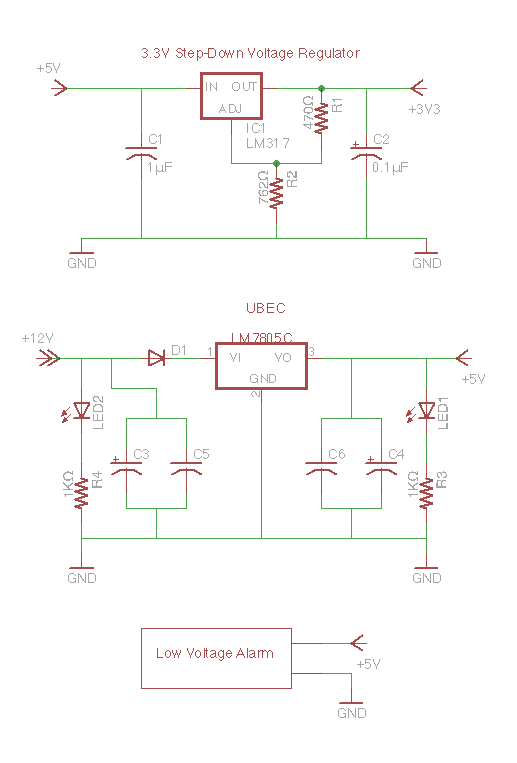
\includegraphics{powerschem}
\caption{Power Conversion Circuits}
\end{center}
\end{figure}

\begin{figure}[htb]
\begin{center}
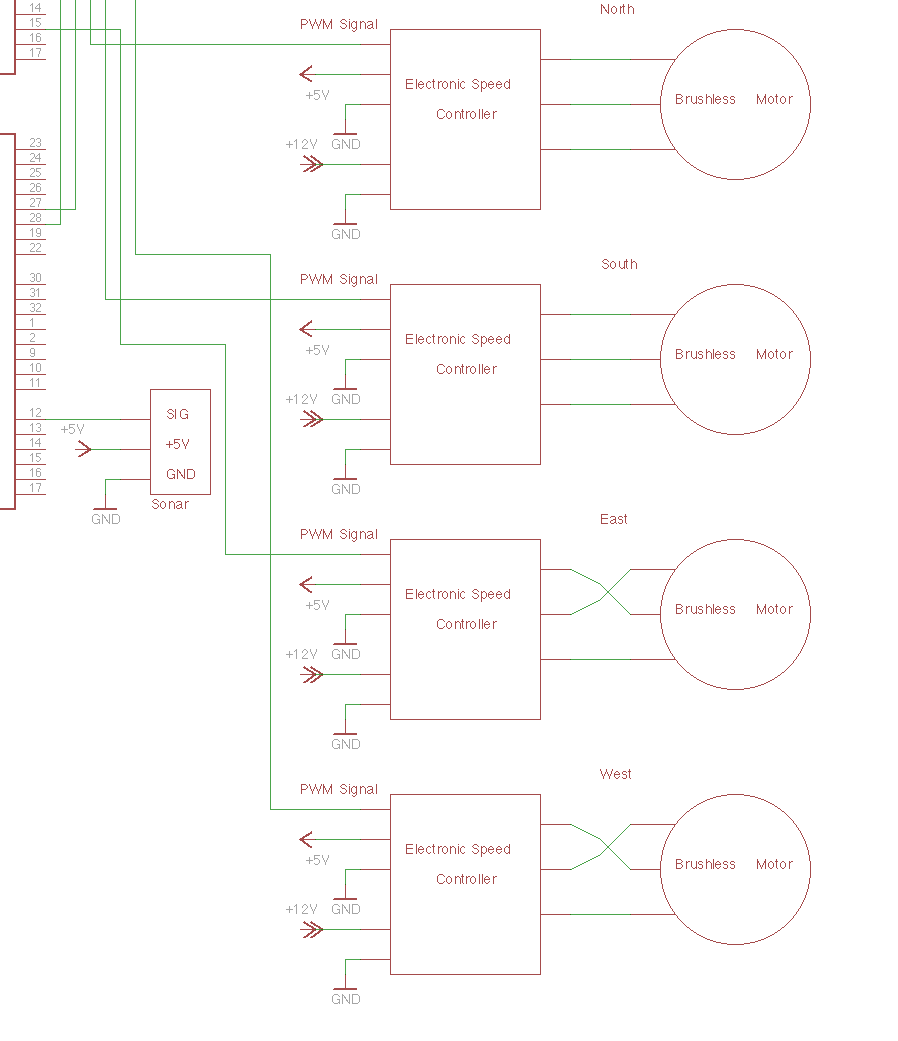
\includegraphics{motorsschem}
\caption{Motor Connections}
\end{center}
\end{figure}

\begin{figure}[htb]
\begin{center}
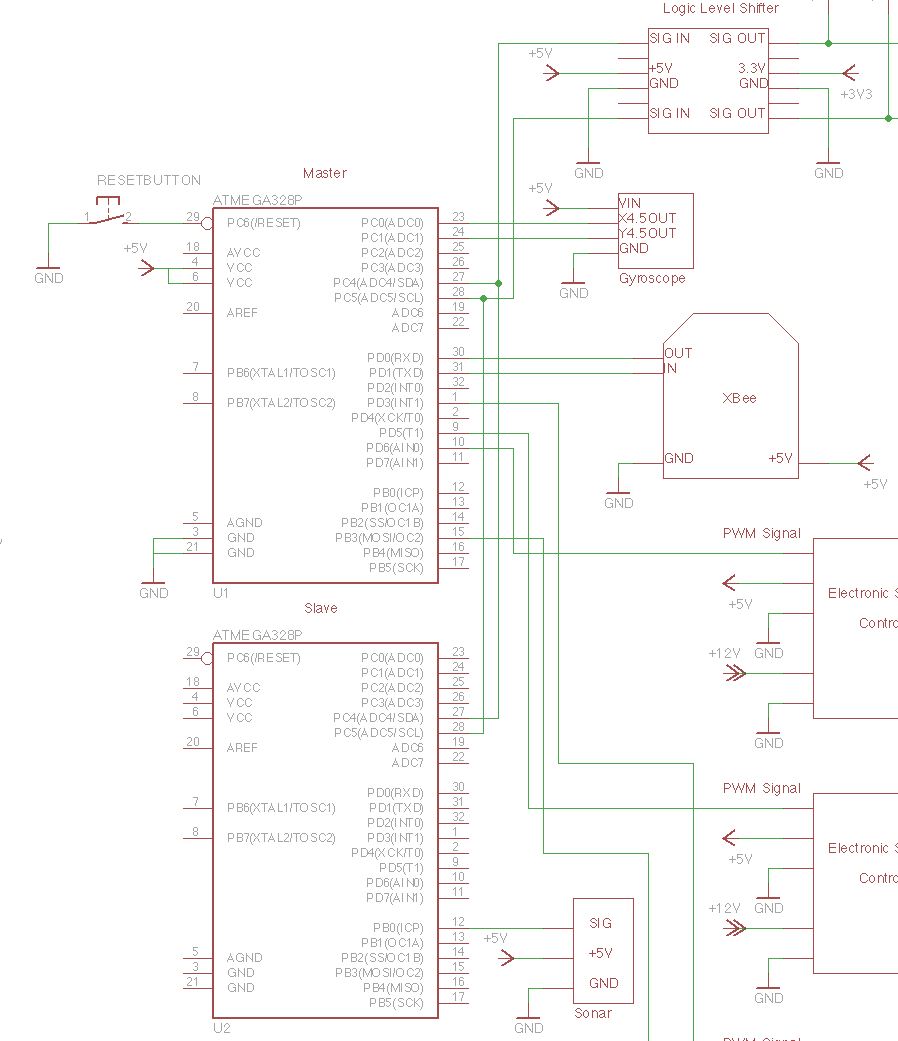
\includegraphics{masterslaveschem}
\caption{AVR Microcontroller Connections}
\end{center}
\end{figure}

\begin{figure}[htb]
\begin{center}
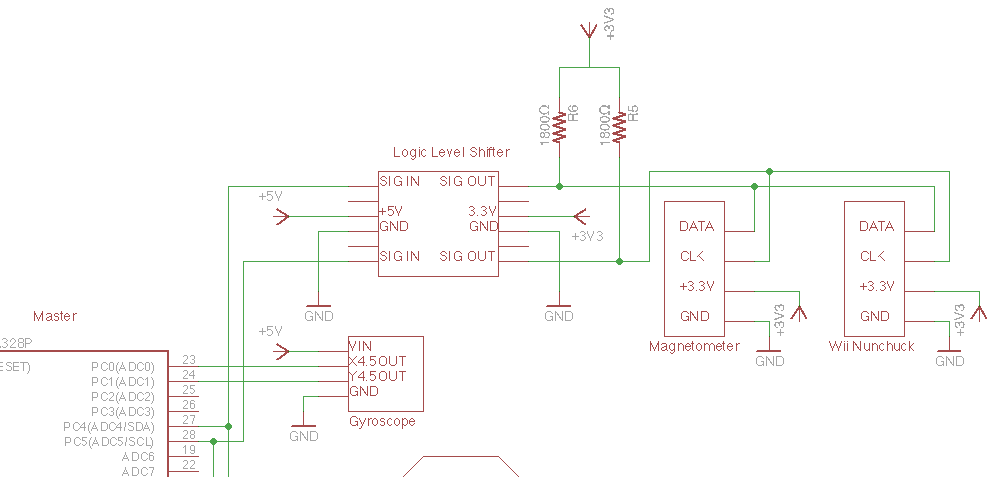
\includegraphics{i2cbusschem}
\caption{$I^2C$ Bus Circuit} 
\end{center}
\end{figure}


\clearpage
\section{Code}



\clearpage
\section{Discussion}
%Discuss Debugging and Improvements


\clearpage
\section{Conclusion}
We built a quadcoptor... I don't really know how to spell that.. 


Equation \ref{eqn} says this
\begin{equation}
says this
\label{eqn}
\end{equation}


% Appendix

\clearpage
\appendix
\appendix
\section{Data Tables}
\setcounter{table}{0}
\renewcommand*\thetable{\Alph{section}.\arabic{table}}
\begin{table}[htpb]
\begin{center}
\caption{Single-Ended CMRR}
\begin{tabular}{|c|c|}
\hline
Frequency (Hz) & CMRR(dB) \\ \hline
1000&	10.972\\ \hline
2000&	10.762\\ \hline
3000&	10.762\\ \hline
4000&	10.762\\ \hline
5000&	10.762\\ \hline
6000&	10.762\\ \hline
7000&	10.762\\ \hline
8000&	10.762\\ \hline
9000&	10.762\\ \hline
10000&	11.003\\ \hline
20000&	10.959\\ \hline
30000&	11.023\\ \hline
40000&	11.126\\ \hline
50000&	11.153\\ \hline
60000&	11.182\\ \hline
70000&	11.346\\ \hline
80000&	11.248\\ \hline
90000&	11.232\\ \hline
100000&	11.377\\ \hline
200000&	11.977\\ \hline
300000&	10.494\\ \hline
400000&	9.542\\ \hline
500000&	9.855\\ \hline
600000&	9.874\\ \hline
700000&	9.588\\ \hline
800000&	6.924\\ \hline
900000&	14.657\\ \hline
1000000&15.398\\ \hline


\end{tabular}
\label{CDgaindata}
\end{center}
\end{table}


% The End
\end{document}
